\iffalse
\begin{table*}[t]
\centering
\caption{\looseness-1Language modeling results on \textsc{WikiText-103}. We use $30\%, 50\%, 70\%$ and $90\%$ of sequences for training in dynamic eval and \textsc{TinT} and the rest of the sequence for evaluation. $\textsc{TinT}$
improves upon the auxiliary model perplexities by $0.3-0.7$ absolute on average.
The small perplexity difference between the \simulator and dynamic evaluation suggests that the approximations introduced in the descent algorithm (\cref{sec:modification}) can still effectively fine-tune the auxiliary model. \sm{Update caption to clearly reference the one-off definition. Change table rows to auxiliray model, one-off dynamic eval, and tint. How many gradient steps is TinT encoding here? Standardize the fonts (small caps vs normal). Check if captions go above or below the table} }
\label{tab:language_modeling}
\begin{tabular}{@{}lcccccccc@{}} \toprule
                 & \multicolumn{4}{c}{\textsc{GPT2}}      & \multicolumn{4}{c}{\textsc{OPT-125m}}  \\ 
              \cmidrule(lr){2-5} \cmidrule(lr){6-9}
Training proportion & $30\%$   & $50\%$   & $70\%$   & $90\%$   & $30\%$   & $50\%$   & $70\%$   & $90\%$   \\ 
\cmidrule(r){1-1} \cmidrule(lr){2-5}\cmidrule(lr){6-9}
\textsc{Vanilla Model}    & 25.6 & 24.9  & 24.5 & 23.3 & 29.6 & 28.8 & 28.0 & 28.0 \\
\textsc{Dyna. FT}     & 24.9 & 24.0    & 23.5 & 22.2 & 29.0 & 28.2 & 27.4 & 27.4 \\
\textsc{TinT}             & 25.1 & 24.3 & 23.8 & 22.6 & 29.3 & 28.4  & 27.5 & 27.4 \\ \bottomrule
\end{tabular}
\end{table*}
\fi





\begin{table}[!t]
\centering
\caption{\looseness-1Language modeling results on \textsc{WikiText-103}. We use $30\%, 50\%, 70\%$ and $90\%$ of sequences for training in the language modeling setting (\textsection{\ref{setting:lm}}). $\textsc{TinT}$
improves the auxiliary model perplexities by $0.3-0.7$ absolute on average.
The small perplexity difference between the \simulator{} and explicitly updating the auxiliary model suggests that the simulated gradient (\cref{sec:modification}) can still effectively fine-tune the auxiliary model. 
%\sm{Update caption to clearly reference the one-off definition. Change table rows to auxiliray model, one-off dynamic eval, and tint. How many gradient steps is TinT encoding here? Standardize the fonts (small caps vs normal). Check if captions go above or below the table} 
}
\label{tab:language_modeling}
\resizebox{\columnwidth}{!}{%
\begin{tabular}{@{}llccccc@{}} \toprule
& & \multicolumn{4}{c}{Training proportion} \\
\cmidrule(lr){3-6} 
& Evaluating with& $30\%$   & $50\%$   & $70\%$   & $90\%$ \\
 % \multicolumn{5}{c}{Auxiliary model: \textsc{GPT2}}    \\ 
 \cmidrule(r){1-2} \cmidrule(lr){3-6}
%\cmidrule(r){1-5}
%                Model & \multicolumn{4}{c}{\textsc{GPT2}}        \\ 
%              \cmidrule(r){1-1} \cmidrule(lr){2-5} 
%\cmidrule(lr){6-9}
\multirow{3}{*}{GPT-2} & \text{Auxiliary Model}    & 25.6 & 24.9  & 24.5 & 23.3 \\
 &\text{Fine-tuning}     & 24.9 & 24.0    & 23.5 & 22.2  \\
 & \simulator{}           & 25.1 & 24.3 & 23.8 & 22.6 \\  
%\midrule
 %\cmidrule(r){1-1} \cmidrule(r){2-5}
%\cmidrule(r){1-1} 
% \cmidrule(r){2-5}
%Model & \multicolumn{4}{c}{\textsc{OPT-125m}} \\
%\cmidrule(r){1-1} \cmidrule(r){2-5}
\cmidrule(r){1-2} \cmidrule(lr){3-6} 
 % \multicolumn{5}{c}{Auxiliary model: \textsc{OPT-125m}} \\
% Auxiliary model: \textsc{OPT-125m}
\multirow{3}{*}{OPT-125M} & \text{Auxiliary Model} & 29.6 & 28.8 & 28.0 & 28.0  \\
& \text{Fine-tuning} & 29.0 & 28.2 & 27.4 & 27.4 \\
& \simulator{}  & 29.3 & 28.4  & 27.5 & 27.4  \\
 \bottomrule
\end{tabular}}
\end{table}


% Our approach provides constructions for diverse variants of pre-trained language models. 
% \Cref{tab:construction} highlights many types of modules and the required size and computation for each.
% %We showcase examples in \Cref{tab:construction} of the types of modules and their required size and computation. 
% The size of a constructed model is influenced by various factors, including the number of layers, and embedding dimension in the auxiliary. 
% We demonstrate the effectiveness of constructed models through language modeling and in-context learning tasks. We evaluate the \simulator{} construction on  \textsc{OPT-125m} model. 


%We conduct experiments to validate the efficacy of our approach. 
%Through these experiments, we demonstrate that the approximations used in constructing the model do not impact model performance.

%We conduct experiments to validate that the approximations introduced (\Cref{sec:modification}) do not significantly harm the capability of \simulator{} to simulate and train an internal model.


% \footnote{Performing many gradient steps can scale the depth of \simulator{} to make the experiments computationally infeasible.}


 \begin{figure*}[t]
    \centering
    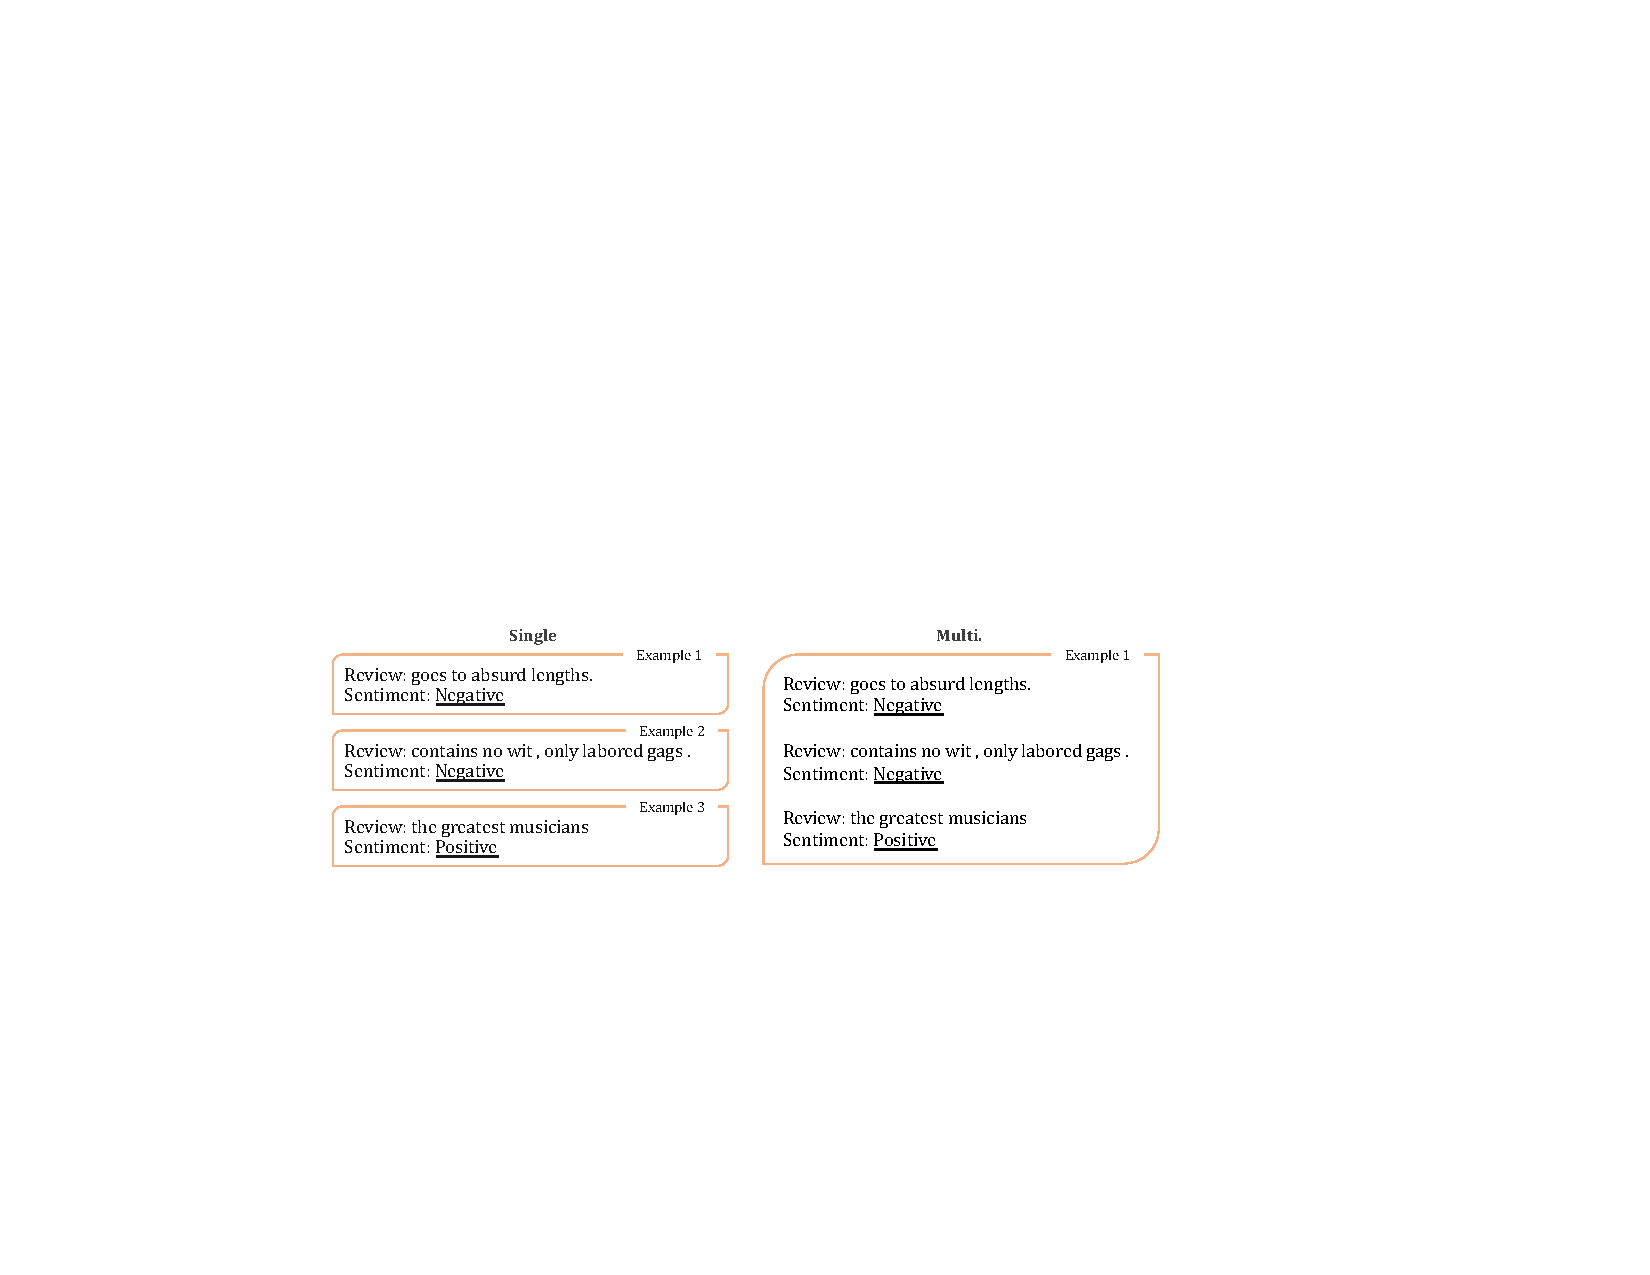
\includegraphics[width=0.75\textwidth]{figures/experiment.pdf}
    \caption{Different settings in few-shot learning ($k=3$) using \simulator{}. The \textbf{Single} mode (left) treats each example as a training datapoint, and the auxiliary model is updated with a batch of inputs (see def.~\ref{def:finetune}). The \textbf{Multi.} mode (right) concatenates all examples to form a single input and uses batch size $1$ in def.~\ref{def:finetune}. For \textbf{Label loss}, only underlined label words are used as training signal, while \textbf{full context loss} includes all tokens.}
    \label{fig:example}
\end{figure*}


\section{Experiments}\label{sec:experiments}

\begin{table*}[t]
  \centering
  \caption{Zero-shot and few-shot in-context learning results across $7$ downstream tasks. All the few-shot results are averaged over three training seeds. \textsc{TinT} consistently surpasses its auxiliary model and achieves comparable performance to one-off dynamic evaluation. \textsc{TinT} outperforms auxiliary models by $3-4\%$ and $12-16\%$ absolute points on average in $0$-shot and  $32$-shot experiments respectively. \textsc{TinT} performs competitively with a similar-sized pre-trained model (\textsc{opt-1.3b}) in both $0$-shot and $32$-shot settings. We show the standard deviation for few-shot settings in parentheses.
  }
  \label{tab:main_result}
  \resizebox{\textwidth}{!}{
  \begin{tabular}{lc|cccccccc}
    \toprule
    \textbf{Model} & \textbf{Shots} & \textbf{Subj} & \textbf{AGNews} & \textbf{SST2} & \textbf{CR} & \textbf{MR} & \textbf{MPQA} & \textbf{Amazon} & \textbf{Avg.} \\
    \midrule
%\multicolumn{2}{c}{} & \multicolumn{8}{c}{\textbf{\textit{Without Calibration}}} \\ %\midrule
\textsc{OPT-125m} & $0$ & $64.0$ & $66.0$ & $70.5$ & $64.5$ & $71.0$ & $68.0$ & $76.5$ & $68.6$ \\
\textsc{OPT-1.3b} & $0$ & $59.0$ & $55.5$ & $54.0$ & $50.5$ & $52.5$ & $74.0$ & $57.0$ & $57.5$ \\
\textsc{OPT-125m} Fine-tuning  & $0$ & $71.0$ & $67.0$ & $79.5$ & $71.5$ & $70.0$ & $68.0$ & $85.5$ & $73.2$ \\
\rowcolor{gray!10}\textsc{OPT-125m TinT} & $0$ & $67.5$ & $66.0$ & $76.5$ & $69.0$ & $76.0$ & $70.5$ & $78.5$ & $72.0$ \\
 \midrule
\textsc{OPT-125m} & $32$ & $58.7_{(4.9)}$ & $33.7_{(8.4)}$ & $50.8_{(1.2)}$ & $51.3_{(1.9)}$ & $50.0_{(0.0)}$ & $54.3_{(2.5)}$ & $55.0_{(6.7)}$ & $50.5_{(1.9)}$ \\
\textsc{OPT-1.3b} & $32$ & $74.2_{(6.1)}$ & $71.3_{(5.3)}$ & $89.8_{(3.6)}$ & $71.5_{(4.5)}$ & $68.3_{(6.1)}$ & $81.7_{(3.3)}$ & $70.3_{(9.9)}$ & $75.3_{(0.4)}$  \\ 
\textsc{OPT-125m} Fine-tuning & $32$ & $78.0_{(1.4)}$ & $66.7_{(1.6)}$ & $71.5_{(1.4)}$ & $73.7_{(3.3)}$ & $72.0_{(0.0)}$ & $80.7_{(0.6)}$ & $79.8_{(0.2)}$ & $74.6_{(2.7)}$ \\
\rowcolor{gray!10}\textsc{OPT-125m TinT} & $32$ & 
$82.3_{(2.7)}$ & $69.3_{(0.9)}$ & $73.7_{(0.8)}$ & $75.7_{(1.9)}$ & $72.3_{(1.2)}$ & $83.2_{(1.0)}$ & $78.2_{(0.2)}$ & $76.4_{(0.7)}$ \\ 
\bottomrule
  \end{tabular}}
\end{table*}


We evaluate the performance of the \simulator{}s constructed using GPT2 and \textsc{OPT-125M} as auxiliary models. 
The findings from our experiments in the  language modeling and in-context learning settings confirm that fine-tuning with the simulated gradients (\Cref{sec:modification}) still allows for effective learning in the auxiliary model.
We loop the training steps (i.e., steps 1-3) outlined in \Cref{sec:design} to accommodate solving real-world natural language tasks.
We formalize the setting below.
%In particular, we allow steps 1-3 (i.e., training the auxiliary model on input data) to be looped.

\subsection{Setting: $N$-step Fine-Tuning}
We formalize the procedure in~\Cref{sec:design} to construct a suitable setting in which we can compare \simulator{} to explicitly training the auxiliary model.
\begin{definition}[$N$-step Fine-Tuning]
    \label{def:finetune}
    Given a batch of training datapoints $\xi_1, \cdots, \xi_B$ and a validation input $\xi'$, we compute and apply gradient updates on the auxiliary model $\aux{\vtheta}$ for timesteps $t=0,...,N-1$ as
    $$ \aux{\vtheta}^{t+1} = \aux{\vtheta}^t - \eta \sum_{i=1}^{B} \nabla_\vtheta \cL(f(\xi_i; \aux{\vtheta}^t)) $$
    where $\eta$ is the learning rate and $\cL$ is a self-supervised loss function on each input $\xi_i$.
    Then, we evaluate the model $\aux{\vtheta}^N$ on $\xi'$.
    $\aux{\vtheta}^0$ denotes the pre-trained auxiliary model.
\end{definition}

Below, we instantiate this setting with text inputs of different formats and different self-supervised loss functions $\cL$. 
To manage computational demands, we limit $N$ to $3$ or fewer.\footnote{Performing many gradient steps scales the depth of \simulator{} and makes experimentation computationally infeasible.} 


\subsection{Case Study: Language Modeling}\label{setting:lm}



The first case we consider is language modeling, where the input data $\ve_1,...,\ve_T$ is natural language without any additional formatting. 
%We consider $\Loss$ to be the self-supervised autoregressive next-token prediction task (\cref{eq:auto_loss}). 
We use a batch size of $1$ in def.~\ref{def:finetune}, and delegate $\xi_1=\ve_1,...,\ve_t$ and $\xi'=\ve_{t+1},...,\ve_T$. 
The loss $\cL$ is the sum of the token-wise autoregressive cross-entropy loss in the sequence $\xi_1$. %\footnote{It is defined as -\sum_{} \log f(x_i) }
%We use the first $t$ tokens as the training data $\xi$, and the rest of the tokens $\ve_{t+1}, \cdots, \ve_T$ as evaluation data $\xi'$. 
For example, given an input \textcolor{red}{Machine learning is a useful tool} \textcolor{brown}{for solving problems.}, we use the \textcolor{red}{red} part as the training data $\xi_1$, and the \textcolor{brown}{brown} part as the validation data $\xi'$. 
We perform language modeling experiments on \textsc{WikiText-103}~\citep{merity2016pointer} and vary the number of tokens $t$ used as training data $\xi$. 

\textbf{Results.}
In \cref{tab:language_modeling}, we observe that \simulator{} achieves a performance comparable to explicit fine-tuning of the auxiliary model, indicating that the simulated gradient~(\Cref{sec:modification}) is largely effective for fine-tuning. Both \simulator{} and explicitly fine-tuning the auxiliary model show improvement over the base model, confirming that minimal tuning on the context indeed enhances predictions on the test portion. 
% \simulator{} achieves lower perplexity lower than the auxiliary model that it was built on. 
\subsection{Case Study: In-Context Learning}
For in-context learning, we consider input data to be a supervised classification task transformed into a next-token prediction task using surrogate labels (see~\Cref{fig:example}). Using binary sentiment classification of movie reviews as an example, given an input (e.g., the review), the model's predicted label is computed as follows. First, we design a simple task-specific prompt (e.g., ``Sentiment:'') and select label words $c_1,...,c_n$ to serve as surrogates for each class (e.g., ``positive'' and ``negative''). Then, we provide the input along with the prompt to the model, and the label assigned the highest probability is treated as the model's prediction.  We describe the zero-shot and few-shot settings below.


\textbf{Zero-shot.}
In the zero-shot setting, we are given text with the first $T-1$ tokens as the input text and final token as the surrogate text label. Hence, we adapt def.~\ref{def:finetune} to use batch size $B=1$, training data $\xi_1=x_1,...,x_{T-1}$, and testing data $\xi' = x_T$.
The loss $\cL$ is again the sum of the token-wise autoregressive cross-entropy losses. 
%\mz{if you move sum of loss to footnote, maybe you need to edit here as well.}

\textbf{Few-shot.}
In the few-shot setting, we are given input texts that are a concatenation of $k$ sequences $\xi_1, \cdots, \xi_k$.
Each sequence contains the input text followed by the surrogate label for the in-context exemplar.
These $k$ exemplars are followed by test data $\xi'$. 
In this case, we can compute the gradient updates to $\aux{\vtheta}$ in two different ways~(\cref{fig:example}). 
The first setting, denoted \textbf{Single}, treats the $k$ sequences as a batch of $B=k$ training datapoints $\xi_1,...,\xi_B$.
The second setting, denoted \textbf{Multi}, treats the concatenation of the $B$ sequences as a single training datapoint $\xi_1$.
%These two settings are referred to as \textbf{Single} and \textbf{Multi} mode setting . 
Furthermore, $\Loss$ for a training datapoint can be defined in two different ways. The first setting, denoted as \textbf{Full context loss}, defines $\Loss$ for a training datapoint $\xi_i$ as the sum of cross entropy loss over all tokens. The second setting, denoted as \textbf{Label loss}, defines $\Loss$ for a training datapoint $\xi_i$ in def. \ref{def:finetune} as the sum of cross entropy loss over the surrogate label tokens.
%or each data point $\zeta_i$, $\netloss$ for a training datapoint $\xi_i$ in \cref{def:finetune} can be defined as the sum of cross entropy loss over all tokens (\textbf{Full context loss}) or the sum of cross entropy loss w.r.t. the surrogate label tokens (\textbf{Label loss}).
%Furthermore, we can make gradient updates in $\aux{\vtheta}$ either using all the tokens in the examples $\xi_1, \cdots, \xi_B$ (\textbf{Full context loss}), or using only the final surrogate tokens in each sequence (\textbf{Label loss}). 
\iffalse

\snote{First we construct a batch of examples with $\xi_1=..., \xi_k=...$. Then $\xi'$ is one test example.}


\paragraph{Loss Functions}
\snote{Regardless of whether we are in the zero-shot or few-shot settings, we can compute the loss in two different ways. These loss functions primarily differ on what tokens they compute the autoregressive cross entropy loss on. Do NOT use ``restricted-context''. Use ``per-example'' or something else. Mengzhou might know a better term.}


% We compare to one-off dynamic evaluation of the auxiliary model. In this setting, the auxiliary model is trained with gradient descent on the training tokens using loss $\Loss$ and evaluated on the validation tokens. The process is independently conducted  across all sequences. This process is equivalent to a one-off version of dynamic evaluation \cite{krause2019dynamic} of the auxiliary model, where in place of increasing prefixes per sequence as training data, we have a one-off split of the input context into training and validation data.

% \begin{definition}[One-off Dynamic evaluation]
%     \label{def:dynamic_eval}
%     For a sequence of $T$ tokens $\ve_1,..,\ve_T$ and hyperparameters $i$ and $\eta$, \emph{one-off dynamic evaluation} of a model $f$ with parameters $\aux{\vtheta}\in\Theta$ and a loss $\Loss$ is defined as follows. 
%     Compute
%     $$ \aux{\vtheta}' = \aux{\vtheta} - \eta\nabla_\theta \Loss(f((\ve_1,...,\ve_i), \aux{\vtheta})).$$
%     Then, the  evaluation loss is $\Loss(f((\ve_{i+1},...,\ve_T), \aux{\vtheta}'))$. 
% \end{definition}

%\paragraph{Loss functions:} Since the construction of \simulator{} allows general context dependent loss functions $\Loss$, we consider the following loss functions $\Loss$ in our experiments and refer to them in the subsequent sections. For subsequent discussion, we assume $f(\xi, \aux{\Theta})$ on a sequence $\xi$ returns the model's predicted probabilities for each prefix context in the sequence $\xi$. For a context $\xi$, we then use $\loss$ to denote the cross entropy loss of prediction of the final token. 

%For the subsequent discussion, we denote $f(\ve_i, \aux{\Theta}; \ve_{j:i-1})$ as the prediction of the we define loss $\loss$ on a token $\ve_i$ in its context $\ve_{j}, \cdots, \ve_{i-1}$ ($j < i$) as the predictive loss of the model $f$ on token $\ve_i$ when presented with the context $\ve_j, \cdots, \ve_{i-1}$. 



\subsection{Setup 1: Language Modeling}
The first case we consider is language modeling, where the input data is natural language without any additional formatting. We consider $\Loss$ to be the self-supervised autoregressive next-token prediction task (\cref{eq:auto_loss}). In this case, the input $\ve_1,...,\ve_T$ is simply an English sentence, where we use the first $t$ tokens as the training data $\xi$, and the rest of the tokens $\ve_{t+1}, \cdots, \ve_T$ to evaluate the updated auxiliary model. For example, given an input \textcolor{red}{Machine learning is a useful tool} \textcolor{brown}{for solving problems.}, we use the \textcolor{red}{red} part as the training data $\xi$, and the \textcolor{brown}{brown} part as the validation data $\xi'$ for \simulator{}. 


%Simulating a more general version of dynamic evaluation is expensive with \simulator{}, as the number of loops over steps 1-3 increases with the number of tokens in $\xi$.
%This process is equivalent to a one-off version of dynamic evaluation \cite{krause2019dynamic} of the auxiliary model, where in place of increasing prefixes per sequence as training data, we have a one-off split of the input context into training and validation data. Simulating a more general version of dynamic evaluation is expensive with \simulator{}, as the number of loops over steps 1-3 increases with the number of tokens in $\xi$. The process of dynamic evaluation is independently conducted  across all sequences.

%In order to evaluate the approximations introduced to gradient descent in \cref{sec:modification}, we compare to one-off evaluation of the auxiliary model.  
%we have a one-off split of the input context into training and validation data.
%\iffalse
\iffalse
\begin{definition}[One-off Dynamic Evaluation]
    \label{def:dynamic_eval}
    For a sequence of $T$ tokens $\ve_1,..,\ve_T$ and hyperparameters $i$ and $\eta$, \emph{dynamic evaluation} of a model $f$ with parameters $\aux{\vtheta}\in\Theta$ and a loss $\Loss$ is defined as follows. 
    %is defined as follows. Let $\Loss: \{\cS, \Theta\}\to \RR$ be a loss function.
    %the cross-entropy language modeling loss. 
    Compute
    $$ \aux{\vtheta}' = \aux{\vtheta} - \eta\nabla_\theta \Loss((\ve_1,...,\ve_i), \aux{\vtheta}).$$
    Then, the  evaluation loss is $\Loss((\ve_{i+1},...,\ve_T), \aux{\vtheta}')$. 
    %For in-context learning, the first $i$ \emph{examples} are used to update the parameters.
\end{definition}
\fi
%\fi 

\iffalse
\begin{definition}[One-off evaluation]
    \label{def:dynamic_eval}
    For a sequence of $T$ tokens $\ve_1,..,\ve_T$ and hyperparameters $i$ and $\eta$, \emph{one-off evaluation loss} of a model $f$ with parameters $\aux{\vtheta}\in\Theta$ and a loss $\Loss$ is defined as follows. 
    %is defined as follows. Let $\Loss: \{\cS, \Theta\}\to \RR$ be a loss function.
    %the cross-entropy language modeling loss. 
    Compute
    $$ \aux{\vtheta}' = \aux{\vtheta} - \eta\nabla_\theta \Loss((\ve_1,...,\ve_i), \aux{\vtheta}).$$
    Then, the  evaluation loss is $\Loss((\ve_{i+1},...,\ve_T), \aux{\vtheta}')$. 
    %For in-context learning, the first $i$ \emph{examples} are used to update the parameters.
\end{definition}
\fi

We perform language modeling experiments on Wikitext-103~\citep{merity2016pointer}. We vary the fraction of  tokens in input sequence used as training data $\xi$ and report the evaluation loss on the rest. %We allow steps 1-3 to be looped for less than $3$ steps, but with the same training data in the sequence, mirroring multi-step evaluation. 
%one-off dynamic evaluation \cite{krause2019dynamic}, where we simply make one context split to create the train and test data for the auxiliary model.
%We compare the performance of \simulator{} to one-off dynamic evaluation \cite{krause2019dynamic}, where we simply make one context split to create the train and test data for the auxiliary model.
%This is equivalent to a one-off dynamic evaluation \cite{krause2019dynamic}, defined as follows.
\iffalse
\begin{definition}[One-off Dynamic Evaluation]
    \label{def:dynamic_eval}
    For a sequence of $T$ tokens $\ve_1,..,\ve_T$ and hyperparameters $i$ and $\eta$, \emph{dynamic evaluation} of a model $f$ with parameters $\aux{\vtheta}\in\Theta$ and a loss $\Loss$ is defined as follows. 
    %is defined as follows. Let $\Loss: \{\cS, \Theta\}\to \RR$ be a loss function.
    %the cross-entropy language modeling loss. 
    Compute
    $$ \aux{\vtheta}' = \aux{\vtheta} - \eta\nabla_\theta \Loss((\ve_1,...,\ve_i), \aux{\vtheta}).$$
    Then, the dynamic evaluation loss is $\Loss((\ve_{i+1},...,\ve_T), \aux{\vtheta}')$. 
    %For in-context learning, the first $i$ \emph{examples} are used to update the parameters.
\end{definition}
\fi
%or example, suppose we perform dynamic evaluation with $i=5$ using the cross-entropy objective on \textcolor{red}{Machine learning is a useful tool} \textcolor{brown}{for solving problems.} The \textcolor{red}{red} part is used to update the pre-trained model, and the \textcolor{brown}{brown} part is used for evaluation. This operation is equivalent to \simulator inference, which implicitly updates a model on the \textcolor{red}{red} portion during the forward pass and then evaluates the updated model on the \textcolor{brown}{brown} portion. Therefore, we use dynamic evaluation as a baseline for \simulator : matching dynamic evaluation performance provides strong evidence that \simulator{}  closely approximates explicitly evaluation the auxiliary model.
%\snote{Make ti clear you're looping through steps 1-3 in Section 2. Step 1 is always on the same input. Include the dynamic evaluation example (and definition) but make sure you tie in the notation of Section 2. One-off dynamic evaluation: just one context split into train and test. Results here. Before the definition, cite the dynamic eval paper and then say that it's prohibitively expensive to take that many gradient steps on every input sequence so we instead formulate the one-off dynamic evaluation.}
\paragraph{Observations:}
In \cref{tab:language_modeling}, we observe  that \simulator{} achieves lower perplexity lower than the auxiliary model that it was built on. Moreover, TINT achieves a performance comparable to one-off dynamic evaluation of the auxiliary model, indicating that the approximations made during its construction largely preserve its effectiveness for fine-tuning. 
\fi 

\textbf{Tasks.} 
We evaluate 7 classification tasks for zero-shot and few-shot settings: 
%For language modeling, we use \textsc{Wikitext-103}~\citep{merity2016pointer}. , we evaluate on $7$ downstream classification tasks: 
\textsc{SST-2} \citep{socher2013recursive}, MR \citep{pang2004sentimental}, CR \citep{hu2004mining}, MPQA \citep{wiebe2005annotating}, Amazon Polarity \citep{zhang2015character}, AGNews \citep{zhang2015character}, and Subj \citep{pang2005seeing}.  


%Our methodology draws inspiration from dynamic evaluation \citep{krause2019dynamic}, where a segment of the input sequence is used to update the auxiliary model, and the remaining portion is used to assess the updated auxiliary model's performance. 



\textbf{Model.} We compare a \simulator{} model that uses an \textsc{OPT-125m} pre-trained model as its auxiliary model against two alternative approaches: (1) directly fine-tuning OPT-125m, and (2) performing standard evaluation using OPT-1.3b, which is of a similar size to \simulator{}.\footnote{Our construction is generally applicable to diverse variants of pre-trained language models (\cref{app:other_construction}).} 





\iffalse
Mathematically, consider an input token sequence $\{s_{t}\}_{t \le T}$. If $\Pr[y \vert \{s_{t}\}_{t \le T}]$ is the model's predicted probability for a given label $y$ and $\Pr[y \vert \Phi]$ is its predicted probability when presented with a simple task-specific context, the model's predicted label on the sequence $\{s_{t}\}_{t \le T}$ with calibration is computed as
\begin{align*}
    \arg\max_y \frac{ \Pr[y \vert \{s_{t}\}_{t \le T}] } {\Pr[y \vert \Phi]}.
\end{align*}
We use $\Phi$ as the set of prompt tokens that we append to each input. For example, in \cref{fig:example}, we use $\Phi$ as the set of tokens involved in the phrase "Sentiment:". 
\fi



\textbf{Observations.} We observe that inferences passes through \simulator{} perform on par with directly fine-tuning the auxiliary model, affirming the validity of the construction design (see~\Cref{sec:design}). As expected, \simulator{} outperforms the base auxiliary model, since it simulates training the auxiliary model. More intriguingly, \simulator{} demonstrates performance comparable to a pre-trained model of similar size (\textsc{OPT-1.3b}). This suggests that the capabilities of existing pre-trained models may be understood via the simulation of smaller auxiliary models. For further details and results of the experiments, please refer to~\Cref{app:experiment}.

%suggesting that standard pre-trained transformer models may inherently employ a similar mechanism to internally train an auxiliary model during inference.



% For downstream tasks (\cref{tab:main_result}), explicit internal training within \simulator{} surpasses vanilla zero-shot evaluation and in-context learning, even with a limited budget of a single forward pass. Moreover, \simulator{} achieves a performance comparable to finetuning the auxiliary model, indicating that the approximations made during its construction largely preserve its effectiveness for fine-tuning. Additionally, we find that \simulator{} outperforms or is on par with a similarly sized pre-trained model (\textsc{opt-1.3b}) . This suggests that the capabilities of existing pre-trained models may be understood via the simulation of smaller auxiliary models. Refer to \cref{app:experiment} for more experiment details and results. 


% We also report the comparisons with calibration in \cref{tab:main_result_app} in the appendix.
